\documentclass[11pt]{article}

\usepackage{amsmath}
\usepackage{amssymb}
\usepackage{fancyhdr}
\usepackage{isotope}
\usepackage{graphicx}
\graphicspath{{./images/}{./}}
\usepackage{array}
\usepackage{caption}
\usepackage{subcaption}

\oddsidemargin0cm
\topmargin-2cm     %I recommend adding these three lines to increase the 
\textwidth16.5cm   %amount of usable space on the page (and save trees)
\textheight23.5cm  

\newcommand{\question}[2] {\vspace{.25in} \hrule\vspace{0.5em}
\noindent{\bf #1: #2} \vspace{0.5em}
\hrule \vspace{.10in}}
\renewcommand{\part}[1] {\vspace{.10in} {\bf (#1)}}

\newcommand{\myname}{Matthew J. Urffer}
\newcommand{\myemail}{murffer@utk.edu}
\newcommand{\myhwnum}{5}
\newcommand{\iso}{\isotope}

\pagestyle{fancyplain}
\lhead{\fancyplain{}{\textbf{HW\myhwnum}}}      % Note the different brackets!
\rhead{\fancyplain{}{\myname\\ \myemail}}
\chead{\fancyplain{}{CHEM-630}}

\begin{document}

\medskip                        % Skip a "medium" amount of space
                                % (latex determines what medium is)
                                % Also try: \bigskip, \littleskip

\thispagestyle{plain}
\begin{center}                  % Center the following lines
{\Large CHEM-630 Assignment \myhwnum} \\
\myname \\
\myemail \\
January 29, 2013 \\
\end{center}

%%%%%%%%%%%%%%%%%%%%%%%%%%%%%%%%%%%%%%%%%%%%%%%%%%%%%%%
\question{2.07}{Radioactivity - Predict Probable Decay}
\part{a}{Predict the probable decay of \iso[55]{Mn}, \iso[123]{Sn}, \iso[66]{Ga}, \iso[185]{Os}, \iso[242]{Pu}, \iso[55]{Fe}, and \iso[249]{Cm}}

\part{b}{Check the above nuclides in a nculide table or chart to see how they actually decay\footnote{Decay schemes for this problem where taken from the Nuclear Data Sheets,2003. (http://www.nndc.bnl.gov/chart/chartNuc.jsp)}}
\begin{center}[hb]
\begin{tabular}{m{1.5cm} m{5.5cm} m{4cm} m{2cm}}
\centering
Isotope & Reason & Predicted Decay Mode & Actual Decay \\
\hline
\hline
\iso[55][25]{Mn} & Odd Z with W-A = 0 &  Stable & Stable \\
\iso[123][50]{Sn} & Even Z with W-A = 4 indicating instability, but Sn has 10 stable isotopes &  Stable & 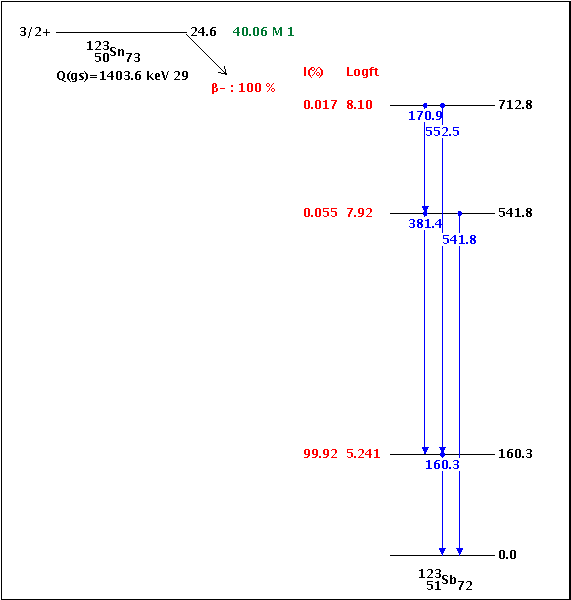
\includegraphics[width=4cm]{123SnDecay.png} \\
\iso[66][31]{Ga} & Odd Z with W-A = -4 indicating instablity with an abudance of neutrons probably $\beta^{-}$ &  $\beta^{-}$ & 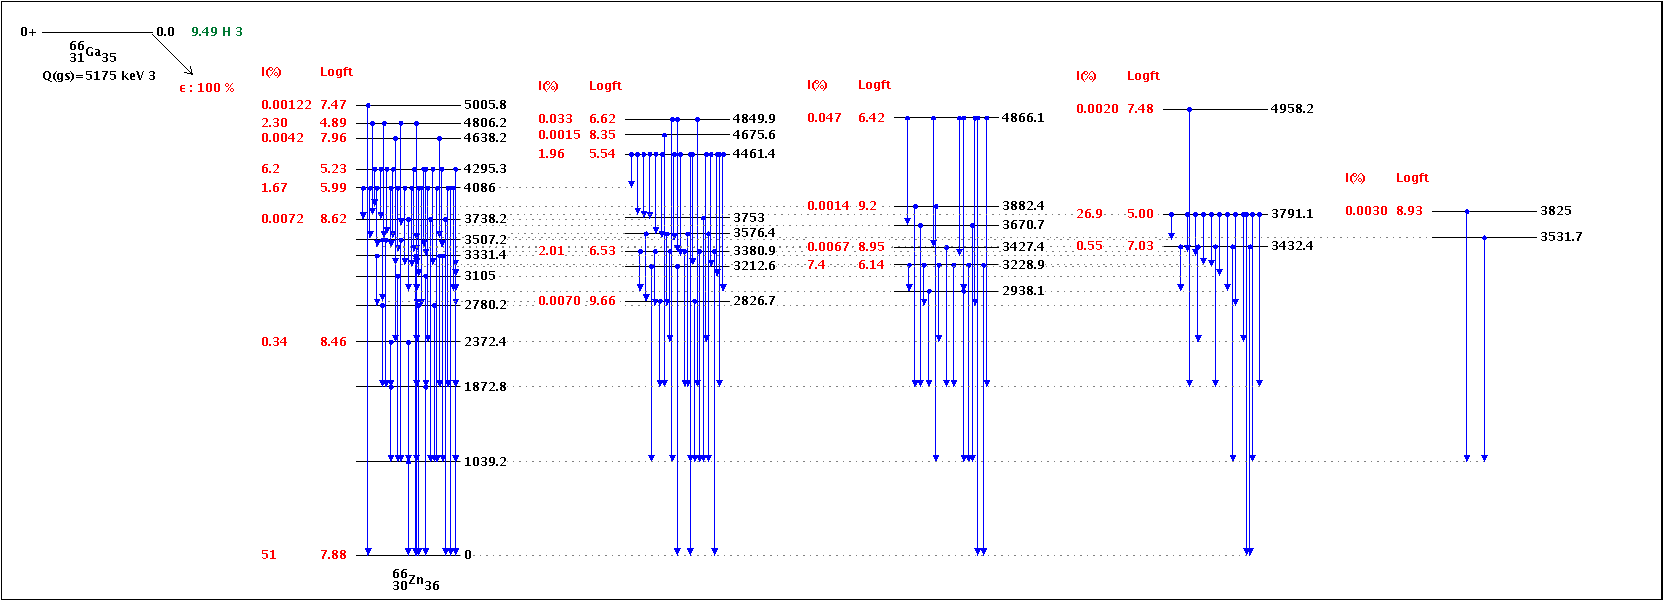
\includegraphics[width=4cm]{66GaDecay.png} \\
\iso[185][76]{Os} & Even Z with W-A = -5 indicating instability with an abudance of neutrons, but probably alpha decay and not beta due to being so far from stability &  $\alpha$ & 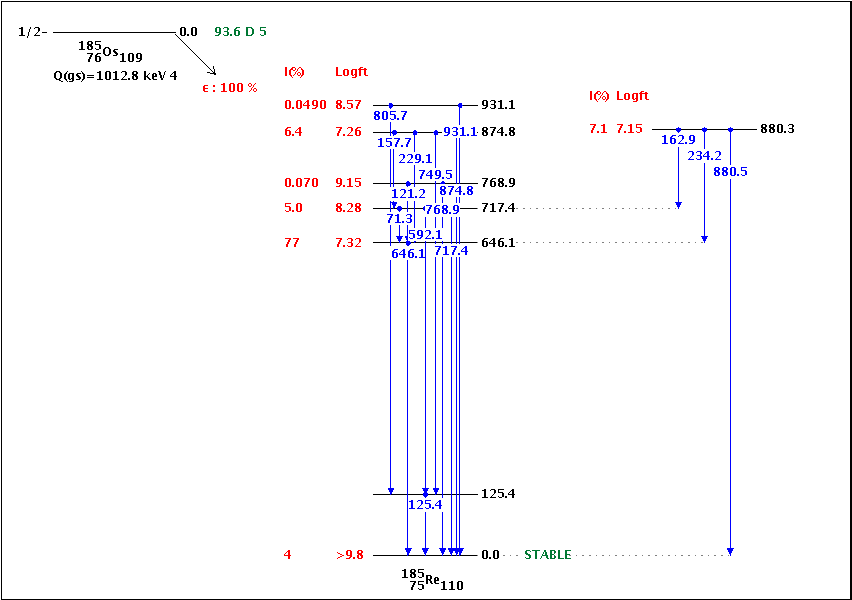
\includegraphics[width=4cm]{185OsDecay.png} \\
\iso[242][94]{Pu} & Even Z with W-A = -2, but all elments above Z=82 are unstable, prediomently through alpha decay &  $\alpha$ & 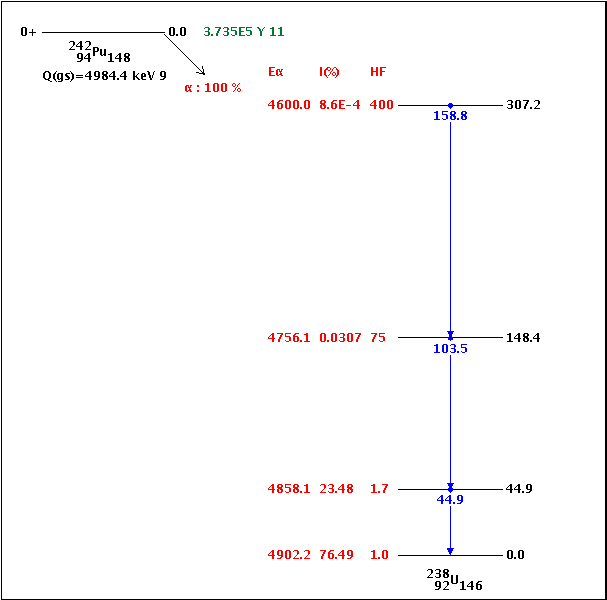
\includegraphics[width=4cm]{242PuDecay.png} \\
\iso[55][26]{Fe} & Even Z with W-A = 1 &  Stable & Estimated half-life is \\
\iso[249][96]{Cm} & Even Z with W-A = 2, but all elments above Z=82 are unstable, prediomently through alpha decay &  $\alpha$ & \includegraphics[width=4cm]{249CmDecay.png} \\
\end{tabular}
\end{center}


%%%%%%%%%%%%%%%%%%%%%%%%%%%%%%%%%%%%%%%%%%%%%%%%%%%%%%%
\question{2.09}{Radioactivity - Reaction Energy}
\part{a}{Calculate the reaction energy invovled in the beta deay of \iso[110]{Ag}}
\begin{align}
	\iso[110][47]{Ag} &\to \iso[110][46]{Pd}^{+} +\beta +\bar{\nu} + Q \\
	Q &= M_{\iso[110]{Ag}} - \left (M_{\iso[110]{Pd}} - M_{e^{-}} + \right ) - M_{e^{-}} - M_{\bar{\nu}} \\
\end{align}
\part{b}{Calculate the reaction energy invovled in the positron decay of \iso[98]{Rh}}
\begin{align}
	\iso[98][45]{Rh} &\to \iso[98][46]{Pd}^{-} + \beta^{+} + \nu + Q \\
	Q &= M_{\iso[98]{Rh}} - \left ( M_{\iso[98]{Pd}} + M_{e^{-}} \right ) - M_{e^{-}} -M_{\nu} \\
\end{align}
\part{c}{Calculate the reaction energy invovled in the electron-capture decay of \iso[111]{Sn}}
\begin{align}
	\iso[110][50]{Sn} + e^{-} &\to \iso[110][49]{In} + \bar{\nu} \\
	Q &= 
\end{align}
\part{d}{Calculate the reaction energy invovled in the alpha decay of \iso[148]{Gd}}
\begin{align}
	\iso[148][64]{Gd} &\to \iso[144][62]{Sm}^{2+} +\alpha^{2-} \\
	Q &= M_{\iso[148]{Gd}} - \left (M_{\iso[114]{Sm}}  + 2m_{e^{-}} \right ) - \left ( M_{\iso[4]{He}} - 2m_{e^{-}} \right ) \\
\end{align}
\part{e}{Calculate the reaction energy invovled in the gamma decay of \iso[107m]{Ag}}

The reaction energy involved in the decay of a meta-stable isotope (such as \iso[107m]{Ag}) cannot be calculated from a mass difference. See the Advanded Topic section for more details.

%%%%%%%%%%%%%%%%%%%%%%%%%%%%%%%%%%%%%%%%%%%%%%%%%%%%%%%
\question{Advanced Topic}{Possible Options}
\begin{itemize}
\item Is it possible (without ruining the state) to observe is an element is meta-stable? What about through it's mass?
\item Is there a relationship between the half-lives and the decay mode?
\item Can a HPGE detector determine the slightly more probable 1.33 MeV gamma
\item Why the extra line in the Th decay diagram?
\end{itemize}

\end{document}

